\documentclass{article}
\usepackage{amsmath, tikz, tkz-graph, tkz-berge}
\usepackage[makeroom]{cancel}
\usetikzlibrary{positioning}
\title{MATH 222 Assignment One}
\author{Oliver Tonnesen\\V00885732}
\date{September 30, 2018}
\begin{document}
\maketitle
\renewcommand{\thesubsection}{\thesection.\alph{subsection}}
\section{} % Section 1
\subsection{}
	Recall that for any graph $G$ on $\ge3$ vertices, if $\deg(v)\ge\frac{n}{2}$ for all v, then $G$ has a Hamiltonian cycle.\\
	$\overline{C_n}=K_n\setminus{C_n}$. Each vertex in $C_n$ has degree $2$, and each vertex in $K_n$ has degree $n-1$, thus removing the
	edges in $C_n$ from $K_n$ leaves each vertex in $K_n$ with $2$ fewer incident edges. So each vertex in $\overline{C_n}$ has degree $n-3$.\\
	We will now find the smallest $n$ for which $\deg(v)\ge\frac{n}{2}$.
	\begin{align*}
		\deg(v)\ge\frac{n}{2}\\
		\deg(v)=n-3\\
		n-3\ge\frac{n}{2}\\
		2n-6\ge{n}\\
		n\ge6
	\end{align*}
	So $\overline{C_n}$ has a Hamiltonian cycle for all $n\ge6$. We can manually check this statement's validity for $n<6$, and find that
	it is true for $n=5$ and false for $n<5$. So $\overline{C_n}$ has a Hamiltonian cycle for $n\ge5$.
\subsection{}
	Colour the graph as so:
	\newline
	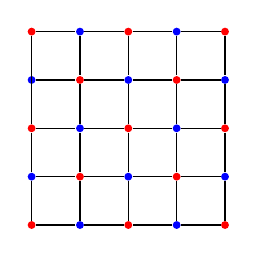
\begin{tikzpicture}[red/.style={circle,fill=red,inner sep=0pt,minimum size=1mm},
						blue/.style={circle,fill=blue,inner sep=0pt,minimum size=1mm}]

		\node[red] 									(00)	{};
		\node[blue,node distance=5mm,below=of 00] 	(10)	{};
		\node[red,node distance=5mm,below=of 10]	(20)	{};
		\node[blue,node distance=5mm,below=of 20] 	(30)	{};
		\node[red,node distance=5mm,below=of 30] 	(40)	{};

		\node[blue,node distance=5mm,right=of 00] 	(01)	{};
		\node[red,node distance=5mm,below=of 01] 	(11)	{};
		\node[blue,node distance=5mm,below=of 11] 	(21)	{};
		\node[red,node distance=5mm,below=of 21] 	(31)	{};
		\node[blue,node distance=5mm,below=of 31] 	(41)	{};

		\node[red,node distance=5mm,right=of 01]	(02)	{};
		\node[blue,node distance=5mm,below=of 02] 	(12)	{};
		\node[red,node distance=5mm,below=of 12] 	(22)	{};
		\node[blue,node distance=5mm,below=of 22] 	(32)	{};
		\node[red,node distance=5mm,below=of 32] 	(42)	{};

		\node[blue,node distance=5mm,right=of 02] 	(03)	{};
		\node[red,node distance=5mm,below=of 03] 	(13)	{};
		\node[blue,node distance=5mm,below=of 13] 	(23)	{};
		\node[red,node distance=5mm,below=of 23] 	(33)	{};
		\node[blue,node distance=5mm,below=of 33] 	(43)	{};

		\node[red,node distance=5mm,right=of 03] 	(04)	{};
		\node[blue,node distance=5mm,below=of 04] 	(14)	{};
		\node[red,node distance=5mm,below=of 14] 	(24)	{};
		\node[blue,node distance=5mm,below=of 24] 	(34)	{};
		\node[red,node distance=5mm,below=of 34] 	(44)	{};

		\draw (00) -- (01);
		\draw (00) -- (20);
		\draw (01) -- (02);
		\draw (01) -- (11);
		\draw (02) -- (03);
		\draw (02) -- (12);
		\draw (03) -- (04);
		\draw (03) -- (13);
		\draw (04) -- (14);
		\draw (14) -- (24);
		\draw (14) -- (13);
		\draw (24) -- (34);
		\draw (34) -- (33);
		\draw (33) -- (43);
		\draw (43) -- (44);
		\draw (44) -- (34);
		\draw (43) -- (42);
		\draw (42) -- (32);
		\draw (32) -- (31);
		\draw (31) -- (41);
		\draw (41) -- (40);
		\draw (41) -- (42);
		\draw (40) -- (30);
		\draw (30) -- (20);
		\draw (30) -- (31);
		\draw (32) -- (33);
		\draw (20) -- (21);
		\draw (21) -- (31);
		\draw (22) -- (32);
		\draw (23) -- (33);
		\draw (21) -- (22);
		\draw (22) -- (23);
		\draw (23) -- (13);
		\draw (23) -- (24);
		\draw (13) -- (12);
		\draw (12) -- (11);
		\draw (12) -- (11);
		\draw (11) -- (10);
		\draw (11) -- (21);
		\draw (12) -- (22);
		\draw (10) -- (00);
	\end{tikzpicture}
	\newline
	\newline
	Note that this graph forms a bipartition. Let $R=\{r\in{V}|\text{$r$ is coloured red}\}$ and $B=\{b\in{V}|\text{$b$ is coloured blue}\}$.\\
	Note that $|R|=36$ and $|B|=40$.\\
	Claim: $G$ does not contain a Hamiltonian cycle.\\
	Proof: (Contradiction)\\
	Suppose there exists a Hamiltonian cycle in $G$. Let this cycle begin in some $v\in{A}$. Then after $2|A|=72$ edges have been traversed,
	we will end up back at $v$. But if only $72$ edges have been traversed, there must still be $4$ vertices in $B$ that have not been visited,
	and so the cycle is not Hamiltonian. This is a contradiction, and so there exists no Hamiltonian cycle in $G$.
\subsection{}
	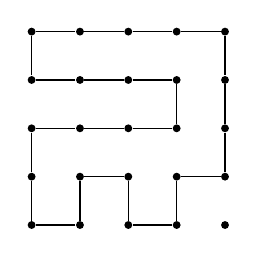
\begin{tikzpicture}[roundnode/.style={circle,fill=black,inner sep=0pt,minimum size=1mm}]
		\node[roundnode] 								(00)	{};
		\node[roundnode,node distance=5mm,below=of 00] 	(10)	{};
		\node[roundnode,node distance=5mm,below=of 10]	(20)	{};
		\node[roundnode,node distance=5mm,below=of 20] 	(30)	{};
		\node[roundnode,node distance=5mm,below=of 30] 	(40)	{};

		\node[roundnode,node distance=5mm,right=of 00] 	(01)	{};
		\node[roundnode,node distance=5mm,below=of 01] 	(11)	{};
		\node[roundnode,node distance=5mm,below=of 11] 	(21)	{};
		\node[roundnode,node distance=5mm,below=of 21] 	(31)	{};
		\node[roundnode,node distance=5mm,below=of 31] 	(41)	{};

		\node[roundnode,node distance=5mm,right=of 01]	(02)	{};
		\node[roundnode,node distance=5mm,below=of 02] 	(12)	{};
		\node[roundnode,node distance=5mm,below=of 12] 	(22)	{};
		\node[roundnode,node distance=5mm,below=of 22] 	(32)	{};
		\node[roundnode,node distance=5mm,below=of 32] 	(42)	{};

		\node[roundnode,node distance=5mm,right=of 02] 	(03)	{};
		\node[roundnode,node distance=5mm,below=of 03] 	(13)	{};
		\node[roundnode,node distance=5mm,below=of 13] 	(23)	{};
		\node[roundnode,node distance=5mm,below=of 23] 	(33)	{};
		\node[roundnode,node distance=5mm,below=of 33] 	(43)	{};

		\node[roundnode,node distance=5mm,right=of 03] 	(04)	{};
		\node[roundnode,node distance=5mm,below=of 04] 	(14)	{};
		\node[roundnode,node distance=5mm,below=of 14] 	(24)	{};
		\node[roundnode,node distance=5mm,below=of 24] 	(34)	{};
		\node[roundnode,node distance=5mm,below=of 34] 	(44)	{};

		\draw (00) -- (01);
		\draw (01) -- (02);
		\draw (02) -- (03);
		\draw (03) -- (04);
		\draw (04) -- (14);
		\draw (14) -- (24);
		\draw (24) -- (34);
		\draw (34) -- (33);
		\draw (33) -- (43);
		\draw (43) -- (42);
		\draw (42) -- (32);
		\draw (32) -- (31);
		\draw (31) -- (41);
		\draw (41) -- (40);
		\draw (40) -- (30);
		\draw (30) -- (20);
		\draw (20) -- (21);
		\draw (21) -- (22);
		\draw (22) -- (23);
		\draw (23) -- (13);
		\draw (13) -- (12);
		\draw (12) -- (11);
		\draw (12) -- (11);
		\draw (11) -- (10);
		\draw (10) -- (00);
	\end{tikzpicture}
	\newline
	There exists no cycle on all $n$ vertices, so this cycle on $n-1$ vertices must be the largest.
\section{} % Section 2
\subsection{}
	$G$ has vertices of degree $3$ \underline{and} $4$, so it must have at least one vertex of each. Consider, then,
	a tree with one vertex of degree $3$, one vertex of degree $4$, and the rest vertices of degree $1$. Let the vertex
	of degree $3$ be the root, and the vertex of degree $4$ one of its children.
	\newline
	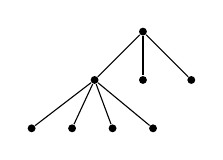
\begin{tikzpicture}[roundnode/.style={circle,fill=black,inner sep=0pt,minimum size=1mm}]
		\node[roundnode]												(00)	{};
		\node[roundnode,node distance=5mm,below=of 00]					(11)	{};
		\node[roundnode,node distance=5mm,left=of 11]					(10)	{};
		\node[roundnode,node distance=5mm,right=of 11]					(12)	{};
		\node[roundnode,node distance=5mm,below=of 10,xshift=-8mm]		(20)	{};
		\node[roundnode,node distance=4mm,right=of 20]					(21)	{};
		\node[roundnode,node distance=4mm,right=of 21]					(22)	{};
		\node[roundnode,node distance=4mm,right=of 22]					(23)	{};

		\draw (00) -- (10);
		\draw (00) -- (11);
		\draw (00) -- (12);
		\draw (10) -- (20);
		\draw (10) -- (21);
		\draw (10) -- (22);
		\draw (10) -- (23);
	\end{tikzpicture}
	\newline
	This tree has $6$ children. The addition of any more non-leaf vertices will never lower the number of leaves,
	so this is the minimal number of leaves in a tree that satisfies the given constraints.
\subsection{}
	Counterexample: $m=3$, $n-4$, $k=1$:
	\newline
	\newline
	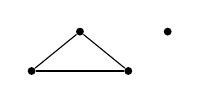
\begin{tikzpicture}[roundnode/.style={circle,fill=black,inner sep=0pt,minimum size=1mm}]
		\node[roundnode]											(0)	{};
		\node[roundnode,node distance=5mm,left=of 0,yshift=-5mm]	(1)	{};
		\node[roundnode,node distance=5mm,right=of 0,yshift=-5mm]	(2)	{};
		\node[roundnode,node distance=10mm,right=of 0]				(3)	{};

		\draw (0) -- (1);
		\draw (0) -- (2);
		\draw (1) -- (2);
	\end{tikzpicture}
	\newline
	\newline
	$0\le3\le4-1$ holds, but the graph has $2$ components despite $k$ being 1. So the claim is false.
\section{} % Section 3
	Recall: For any connected plane graph, $n-m+r=2$ and $m\le3n-6$.
	\begin{align*}
		n-m+r&=2\\
		n-m+96&=2\qquad&\text{($r=96$)}\\
		n-m&=-94\\
		n-(3n-6)&\ge-94\qquad&\text{($m\le3n-6$)}\\
		-2n+6&\ge-94\\
		2n&\ge100\\
		n&\ge50
	\end{align*}
	So the graph must have at least $n$ vertices.
\section{} % Section 4
	\begin{minipage}{.45\textwidth}
		\centering
		$G$:
		\newline
		\newline
		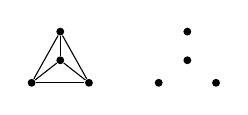
\begin{tikzpicture}[roundnode/.style={circle,fill=black,inner sep=0pt,minimum size=1mm}]
			\node[roundnode]												(l0)	{};
			\node[roundnode,node distance=2.5mm,below=of l0]				(l1)	{};
			\node[roundnode,node distance=2.5mm,left=of l0,yshift=-6.5mm]	(l2)	{};
			\node[roundnode,node distance=2.5mm,right=of l0,yshift=-6.5mm]	(l3)	{};

			\node[roundnode,node distance=15mm,right=of l0]					(r0)	{};
			\node[roundnode,node distance=2.5mm,below=of r0]				(r1)	{};
			\node[roundnode,node distance=2.5mm,left=of r0,yshift=-6.5mm]	(r2)	{};
			\node[roundnode,node distance=2.5mm,right=of r0,yshift=-6.5mm]	(r3)	{};

			\draw (l0) -- (l1);
			\draw (l0) -- (l2);
			\draw (l0) -- (l3);
			\draw (l1) -- (l2);
			\draw (l1) -- (l3);
			\draw (l2) -- (l3);
		\end{tikzpicture}
	\end{minipage}
	\begin{minipage}{.45\textwidth}
		\centering
		$\overline{G}$:
		\newline
		\newline
		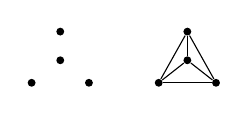
\begin{tikzpicture}[roundnode/.style={circle,fill=black,inner sep=0pt,minimum size=1mm}]
			\node[roundnode]												(l0)	{};
			\node[roundnode,node distance=2.5mm,below=of l0]				(l1)	{};
			\node[roundnode,node distance=2.5mm,left=of l0,yshift=-6.5mm]	(l2)	{};
			\node[roundnode,node distance=2.5mm,right=of l0,yshift=-6.5mm]	(l3)	{};

			\node[roundnode,node distance=15mm,right=of l0]					(r0)	{};
			\node[roundnode,node distance=2.5mm,below=of r0]				(r1)	{};
			\node[roundnode,node distance=2.5mm,left=of r0,yshift=-6.5mm]	(r2)	{};
			\node[roundnode,node distance=2.5mm,right=of r0,yshift=-6.5mm]	(r3)	{};

			\draw (r0) -- (r1);
			\draw (r0) -- (r2);
			\draw (r0) -- (r3);
			\draw (r1) -- (r2);
			\draw (r1) -- (r3);
			\draw (r2) -- (r3);
		\end{tikzpicture}
	\end{minipage}
\section{} % Section 5
	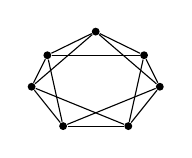
\begin{tikzpicture}[roundnode/.style={circle,fill=black,inner sep=0pt,minimum size=1mm}]
		\node[roundnode]											(1)		{};
		\node[roundnode,node distance=5mm,left=of 1,yshift=-3mm]	(2)		{};
		\node[roundnode,node distance=5mm,right=of 1,yshift=-3mm]	(3)		{};
		\node[roundnode,node distance=7mm,left=of 1,yshift=-7mm]	(4)		{};
		\node[roundnode,node distance=7mm,right=of 1,yshift=-7mm]	(5)		{};
		\node[roundnode,node distance=3mm,left=of 1,yshift=-12mm]	(6)		{};
		\node[roundnode,node distance=3mm,right=of 1,yshift=-12mm]	(7)		{};

		\draw (1) -- (2);
		\draw (1) -- (3);
		\draw (1) -- (4);
		\draw (1) -- (5);
		\draw (2) -- (3);
		\draw (2) -- (4);
		\draw (2) -- (6);
		\draw (3) -- (5);
		\draw (3) -- (7);
		\draw (4) -- (6);
		\draw (4) -- (7);
		\draw (5) -- (6);
		\draw (5) -- (7);
		\draw (6) -- (7);
	\end{tikzpicture}
	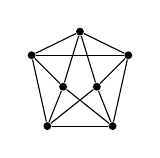
\begin{tikzpicture}[roundnode/.style={circle,fill=black,inner sep=0pt,minimum size=1mm}]
		\node[roundnode]														(1)		{};
		\node[roundnode,node distance=5mm,left=of 1,yshift=-3mm]				(2)		{};
		\node[roundnode,node distance=5mm,right=of 1,yshift=-3mm]				(3)		{};
		\node[roundnode,node distance=1mm,left=of 1,yshift=-7mm]				(4)		{};
		\node[roundnode,node distance=1mm,right=of 1,yshift=-7mm]				(5)		{};
		\node[roundnode,node distance=3mm,left=of 1,yshift=-12mm]				(6)		{};
		\node[roundnode,node distance=3mm,right=of 1,yshift=-12mm]				(7)		{};

		\draw (1) -- (2);
		\draw (1) -- (3);
		\draw (1) -- (4);
		\draw (1) -- (5);
		\draw (2) -- (3);
		\draw (2) -- (4);
		\draw (2) -- (6);
		\draw (3) -- (5);
		\draw (3) -- (7);
		\draw (4) -- (6);
		\draw (4) -- (7);
		\draw (5) -- (6);
		\draw (5) -- (7);
		\draw (6) -- (7);
	\end{tikzpicture}
	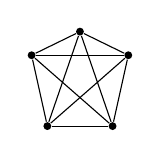
\begin{tikzpicture}[roundnode/.style={circle,fill=black,inner sep=0pt,minimum size=1mm}]
		\node[roundnode]														(1)		{};
		\node[roundnode,node distance=5mm,left=of 1,yshift=-3mm]				(2)		{};
		\node[roundnode,node distance=5mm,right=of 1,yshift=-3mm]				(3)		{};
		\node[roundnode,node distance=3mm,left=of 1,yshift=-12mm]				(6)		{};
		\node[roundnode,node distance=3mm,right=of 1,yshift=-12mm]				(7)		{};

		\draw (1) -- (2);
		\draw (1) -- (3);
		\draw (1) -- (6);
		\draw (1) -- (7);
		\draw (2) -- (3);
		\draw (2) -- (7);
		\draw (2) -- (6);
		\draw (3) -- (6);
		\draw (3) -- (7);
		\draw (6) -- (7);
	\end{tikzpicture}
	\newline
	\newline
	\newline
	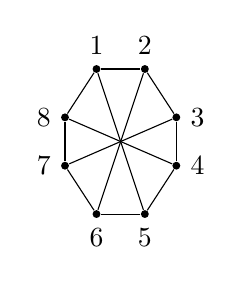
\begin{tikzpicture}[roundnode/.style={circle,fill=black,inner sep=0pt,minimum size=1mm}]
		\node[roundnode,label={90:1}]											(1)		{};
		\node[roundnode,node distance=5mm,right=of 1,label={90:2}]				(2)		{};
		\node[roundnode,node distance=5mm,below=of 2,xshift=4mm,label={0:3}]	(3)		{};
		\node[roundnode,node distance=5mm,below=of 3,label={0:4}]				(4)		{};
		\node[roundnode,node distance=5mm,below=of 4,xshift=-4mm,label={270:5}]	(5)		{};
		\node[roundnode,node distance=5mm,left=of 5,label={270:6}]				(6)		{};
		\node[roundnode,node distance=5mm,above=of 6,xshift=-4mm,label={180:7}]	(7)		{};
		\node[roundnode,node distance=5mm,above=of 7,label={180:8}]				(8)		{};

		\draw (1) -- (2);
		\draw (1) -- (5);
		\draw (1) -- (8);
		\draw (2) -- (3);
		\draw (2) -- (6);
		\draw (3) -- (4);
		\draw (3) -- (7);
		\draw (4) -- (5);
		\draw (4) -- (8);
		\draw (5) -- (6);
		\draw (6) -- (7);
		\draw (7) -- (8);
	\end{tikzpicture}
	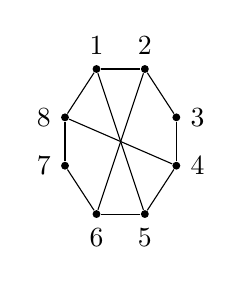
\begin{tikzpicture}[roundnode/.style={circle,fill=black,inner sep=0pt,minimum size=1mm}]
		\node[roundnode,label={90:1}]											(1)		{};
		\node[roundnode,node distance=5mm,right=of 1,label={90:2}]				(2)		{};
		\node[roundnode,node distance=5mm,below=of 2,xshift=4mm,label={0:3}]	(3)		{};
		\node[roundnode,node distance=5mm,below=of 3,label={0:4}]				(4)		{};
		\node[roundnode,node distance=5mm,below=of 4,xshift=-4mm,label={270:5}]	(5)		{};
		\node[roundnode,node distance=5mm,left=of 5,label={270:6}]				(6)		{};
		\node[roundnode,node distance=5mm,above=of 6,xshift=-4mm,label={180:7}]	(7)		{};
		\node[roundnode,node distance=5mm,above=of 7,label={180:8}]				(8)		{};

		\draw (1) -- (2);
		\draw (1) -- (5);
		\draw (1) -- (8);
		\draw (2) -- (3);
		\draw (2) -- (6);
		\draw (3) -- (4);
		\draw (4) -- (5);
		\draw (4) -- (8);
		\draw (5) -- (6);
		\draw (6) -- (7);
		\draw (7) -- (8);
	\end{tikzpicture}
	\begin{tikzpicture}[roundnode/.style={circle,fill=black,inner sep=0pt,minimum size=1mm}]
		\node[roundnode,label={90:1}]											(1)		{};
		\node[roundnode,node distance=5mm,right=of 1,label={90:2}]				(2)		{};
		\node[roundnode,node distance=5mm,below=of 3,label={0:4}]				(4)		{};
		\node[roundnode,node distance=5mm,below=of 4,xshift=-4mm,label={270:5}]	(5)		{};
		\node[roundnode,node distance=5mm,left=of 5,label={270:6}]				(6)		{};
		\node[roundnode,node distance=5mm,above=of 7,label={180:8}]				(8)		{};

		\draw (1) -- (2);
		\draw (1) -- (5);
		\draw (1) -- (8);
		\draw (2) -- (4);
		\draw (2) -- (6);
		\draw (4) -- (5);
		\draw (4) -- (8);
		\draw (5) -- (6);
		\draw (6) -- (8);
	\end{tikzpicture}
	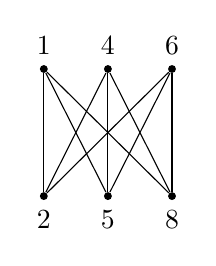
\begin{tikzpicture}[roundnode/.style={circle,fill=black,inner sep=0pt,minimum size=1mm}]
		\node[roundnode,label={90:1}]									(1)		{};
		\node[roundnode,node distance=7mm,right=of 1,label={90:4}]		(4)		{};
		\node[roundnode,node distance=7mm,right=of 4,label={90:6}]		(6)		{};

		\node[roundnode,node distance=15mm,below=of 1,label={270:2}]	(2)		{};
		\node[roundnode,node distance=7mm,right=of 2,label={270:5}]		(5)		{};
		\node[roundnode,node distance=7mm,right=of 5,label={270:8}]		(8)		{};

		\draw (1) -- (2);
		\draw (1) -- (5);
		\draw (1) -- (8);
		\draw (2) -- (4);
		\draw (2) -- (6);
		\draw (4) -- (5);
		\draw (4) -- (8);
		\draw (5) -- (6);
		\draw (6) -- (8);
	\end{tikzpicture}
\section{} % Section 6
	Note that the first graph has $C_7$ as a subgraph, and so its chromatic number must be at least 3.\\
	We will now attempt to construct a 4-colouring for this graph:
	\newline
	\newline
	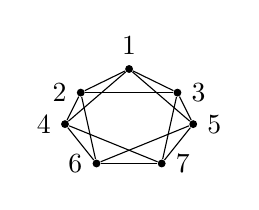
\begin{tikzpicture}[red/.style={circle,fill=red,inner sep=0pt,minimum size=1mm},
						blue/.style={circle,fill=blue,inner sep=0pt,minimum size=1mm},
						green/.style={circle,fill=green,inner sep=0pt,minimum size=1mm},
						black/.style={circle,fill=black,inner sep=0pt,minimum size=1mm}]
		\node[black,label={90:1}]											(1)		{};
		\node[black,node distance=5mm,left=of 1,yshift=-3mm,label={180:2}]	(2)		{};
		\node[black,node distance=5mm,right=of 1,yshift=-3mm,label={0:3}]	(3)		{};
		\node[black,node distance=7mm,left=of 1,yshift=-7mm,label={180:4}]	(4)		{};
		\node[black,node distance=7mm,right=of 1,yshift=-7mm,label={0:5}]	(5)		{};
		\node[black,node distance=3mm,left=of 1,yshift=-12mm,label={180:6}]	(6)		{};
		\node[black,node distance=3mm,right=of 1,yshift=-12mm,label={0:7}]	(7)		{};

		\draw (1) -- (2);
		\draw (1) -- (3);
		\draw (1) -- (4);
		\draw (1) -- (5);
		\draw (2) -- (3);
		\draw (2) -- (4);
		\draw (2) -- (6);
		\draw (3) -- (5);
		\draw (3) -- (7);
		\draw (4) -- (6);
		\draw (4) -- (7);
		\draw (5) -- (6);
		\draw (5) -- (7);
		\draw (6) -- (7);
	\end{tikzpicture}
	\newline
	\newline
	Consider the three copies of $K_3$: $\{1,2,3\}$, $\{1,3,5\}$, and $\{2,4,6\}$. Note that each vertex must not share its colour within the set.
	We will try to colour the vertices in each triangle
	\newline
	\newline
	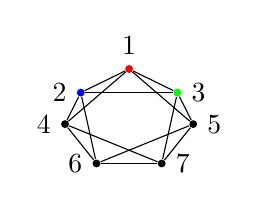
\begin{tikzpicture}[red/.style={circle,fill=red,inner sep=0pt,minimum size=1mm},
						blue/.style={circle,fill=blue,inner sep=0pt,minimum size=1mm},
						green/.style={circle,fill=green,inner sep=0pt,minimum size=1mm},
						black/.style={circle,fill=black,inner sep=0pt,minimum size=1mm}]
		\node[red,label={90:1}]											(1)		{};
		\node[blue,node distance=5mm,left=of 1,yshift=-3mm,label={180:2}]	(2)		{};
		\node[green,node distance=5mm,right=of 1,yshift=-3mm,label={0:3}]	(3)		{};
		\node[black,node distance=7mm,left=of 1,yshift=-7mm,label={180:4}]	(4)		{};
		\node[black,node distance=7mm,right=of 1,yshift=-7mm,label={0:5}]	(5)		{};
		\node[black,node distance=3mm,left=of 1,yshift=-12mm,label={180:6}]	(6)		{};
		\node[black,node distance=3mm,right=of 1,yshift=-12mm,label={0:7}]	(7)		{};

		\draw (1) -- (2);
		\draw (1) -- (3);
		\draw (1) -- (4);
		\draw (1) -- (5);
		\draw (2) -- (3);
		\draw (2) -- (4);
		\draw (2) -- (6);
		\draw (3) -- (5);
		\draw (3) -- (7);
		\draw (4) -- (6);
		\draw (4) -- (7);
		\draw (5) -- (6);
		\draw (5) -- (7);
		\draw (6) -- (7);
	\end{tikzpicture}
	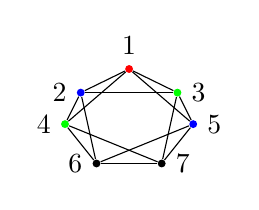
\begin{tikzpicture}[red/.style={circle,fill=red,inner sep=0pt,minimum size=1mm},
						blue/.style={circle,fill=blue,inner sep=0pt,minimum size=1mm},
						green/.style={circle,fill=green,inner sep=0pt,minimum size=1mm},
						black/.style={circle,fill=black,inner sep=0pt,minimum size=1mm}]
		\node[red,label={90:1}]											(1)		{};
		\node[blue,node distance=5mm,left=of 1,yshift=-3mm,label={180:2}]	(2)		{};
		\node[green,node distance=5mm,right=of 1,yshift=-3mm,label={0:3}]	(3)		{};
		\node[green,node distance=7mm,left=of 1,yshift=-7mm,label={180:4}]	(4)		{};
		\node[blue,node distance=7mm,right=of 1,yshift=-7mm,label={0:5}]	(5)		{};
		\node[black,node distance=3mm,left=of 1,yshift=-12mm,label={180:6}]	(6)		{};
		\node[black,node distance=3mm,right=of 1,yshift=-12mm,label={0:7}]	(7)		{};

		\draw (1) -- (2);
		\draw (1) -- (3);
		\draw (1) -- (4);
		\draw (1) -- (5);
		\draw (2) -- (3);
		\draw (2) -- (4);
		\draw (2) -- (6);
		\draw (3) -- (5);
		\draw (3) -- (7);
		\draw (4) -- (6);
		\draw (4) -- (7);
		\draw (5) -- (6);
		\draw (5) -- (7);
		\draw (6) -- (7);
	\end{tikzpicture}
	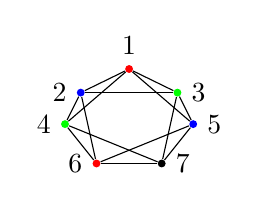
\begin{tikzpicture}[red/.style={circle,fill=red,inner sep=0pt,minimum size=1mm},
						blue/.style={circle,fill=blue,inner sep=0pt,minimum size=1mm},
						green/.style={circle,fill=green,inner sep=0pt,minimum size=1mm},
						black/.style={circle,fill=black,inner sep=0pt,minimum size=1mm}]
		\node[red,label={90:1}]											(1)		{};
		\node[blue,node distance=5mm,left=of 1,yshift=-3mm,label={180:2}]	(2)		{};
		\node[green,node distance=5mm,right=of 1,yshift=-3mm,label={0:3}]	(3)		{};
		\node[green,node distance=7mm,left=of 1,yshift=-7mm,label={180:4}]	(4)		{};
		\node[blue,node distance=7mm,right=of 1,yshift=-7mm,label={0:5}]	(5)		{};
		\node[red,node distance=3mm,left=of 1,yshift=-12mm,label={180:6}]	(6)		{};
		\node[black,node distance=3mm,right=of 1,yshift=-12mm,label={0:7}]	(7)		{};

		\draw (1) -- (2);
		\draw (1) -- (3);
		\draw (1) -- (4);
		\draw (1) -- (5);
		\draw (2) -- (3);
		\draw (2) -- (4);
		\draw (2) -- (6);
		\draw (3) -- (5);
		\draw (3) -- (7);
		\draw (4) -- (6);
		\draw (4) -- (7);
		\draw (5) -- (6);
		\draw (5) -- (7);
		\draw (6) -- (7);
	\end{tikzpicture}
	\newline
	\newline
	The rest of the graph cannot be coloured any differently; each copy of $K_3$ must have 3 distinct colours. So there exists no 3-colouring for this graph.
	We will now provide a 4-colouring for this graph.
	\newline
	\newline
	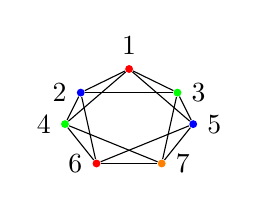
\begin{tikzpicture}[red/.style={circle,fill=red,inner sep=0pt,minimum size=1mm},
						blue/.style={circle,fill=blue,inner sep=0pt,minimum size=1mm},
						green/.style={circle,fill=green,inner sep=0pt,minimum size=1mm},
						orange/.style={circle,fill=orange,inner sep=0pt,minimum size=1mm}]
		\node[red,label={90:1}]											(1)		{};
		\node[blue,node distance=5mm,left=of 1,yshift=-3mm,label={180:2}]	(2)		{};
		\node[green,node distance=5mm,right=of 1,yshift=-3mm,label={0:3}]	(3)		{};
		\node[green,node distance=7mm,left=of 1,yshift=-7mm,label={180:4}]	(4)		{};
		\node[blue,node distance=7mm,right=of 1,yshift=-7mm,label={0:5}]	(5)		{};
		\node[red,node distance=3mm,left=of 1,yshift=-12mm,label={180:6}]	(6)		{};
		\node[orange,node distance=3mm,right=of 1,yshift=-12mm,label={0:7}]	(7)		{};

		\draw (1) -- (2);
		\draw (1) -- (3);
		\draw (1) -- (4);
		\draw (1) -- (5);
		\draw (2) -- (3);
		\draw (2) -- (4);
		\draw (2) -- (6);
		\draw (3) -- (5);
		\draw (3) -- (7);
		\draw (4) -- (6);
		\draw (4) -- (7);
		\draw (5) -- (6);
		\draw (5) -- (7);
		\draw (6) -- (7);
	\end{tikzpicture}
	\newline
	\newline
	So this first graph's chromatic number is 4.
	\newline
	For the second graph, we shall first prove that there exists no 2-colouring, and then provide a 3-colouring to prove its existence.\\
	Suppose there exists a 2-colouring of the graph. Then its outer edges forming $C_8$ must be coloured as so:
	\newline
	\newline
	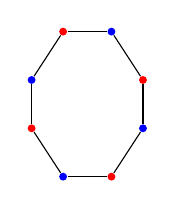
\begin{tikzpicture}[red/.style={circle,fill=red,inner sep=0pt,minimum size=1mm},blue/.style={circle,fill=blue,inner sep=0pt,minimum size=1mm}]
		\node[red]											(1)		{};
		\node[blue,node distance=5mm,right=of 1]			(2)		{};
		\node[red,node distance=5mm,below=of 2,xshift=4mm]	(3)		{};
		\node[blue,node distance=5mm,below=of 3]			(4)		{};
		\node[red,node distance=5mm,below=of 4,xshift=-4mm]	(5)		{};
		\node[blue,node distance=5mm,left=of 5]				(6)		{};
		\node[red,node distance=5mm,above=of 6,xshift=-4mm]	(7)		{};
		\node[blue,node distance=5mm,above=of 7]			(8)		{};

		\draw (1) -- (2);
		\draw (2) -- (3);
		\draw (3) -- (4);
		\draw (4) -- (5);
		\draw (5) -- (6);
		\draw (6) -- (7);
		\draw (7) -- (8);
		\draw (8) -- (1);
	\end{tikzpicture}
	\newline
	\newline
	If we now insert the rest of the edges belonging to the original graph, we find that there are edges connected red vertices to red vertices
	and blue vertices to blue vertices:
	\newline
	\newline
	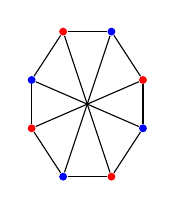
\begin{tikzpicture}[red/.style={circle,fill=red,inner sep=0pt,minimum size=1mm},blue/.style={circle,fill=blue,inner sep=0pt,minimum size=1mm}]
		\node[red]											(1)		{};
		\node[blue,node distance=5mm,right=of 1]			(2)		{};
		\node[red,node distance=5mm,below=of 2,xshift=4mm]	(3)		{};
		\node[blue,node distance=5mm,below=of 3]			(4)		{};
		\node[red,node distance=5mm,below=of 4,xshift=-4mm]	(5)		{};
		\node[blue,node distance=5mm,left=of 5]				(6)		{};
		\node[red,node distance=5mm,above=of 6,xshift=-4mm]	(7)		{};
		\node[blue,node distance=5mm,above=of 7]			(8)		{};

		\draw (1) -- (2);
		\draw (1) -- (5);
		\draw (1) -- (8);
		\draw (2) -- (3);
		\draw (2) -- (6);
		\draw (3) -- (4);
		\draw (3) -- (7);
		\draw (4) -- (5);
		\draw (4) -- (8);
		\draw (5) -- (6);
		\draw (6) -- (7);
		\draw (7) -- (8);
	\end{tikzpicture}
	\newline
	\newline
	This is a contradiction, and so there is no 2-colouring for the graph. We now provide a 3-colouring:
	\newline
	\newline
	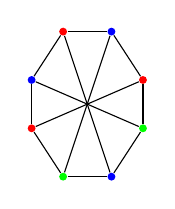
\begin{tikzpicture}[red/.style={circle,fill=red,inner sep=0pt,minimum size=1mm},blue/.style={circle,fill=blue,inner sep=0pt,minimum size=1mm},green/.style={circle,fill=green,inner sep=0pt,minimum size=1mm}]
		\node[red]											(1)		{};
		\node[blue,node distance=5mm,right=of 1]			(2)		{};
		\node[red,node distance=5mm,below=of 2,xshift=4mm]	(3)		{};
		\node[green,node distance=5mm,below=of 3]			(4)		{};
		\node[blue,node distance=5mm,below=of 4,xshift=-4mm]	(5)		{};
		\node[green,node distance=5mm,left=of 5]				(6)		{};
		\node[red,node distance=5mm,above=of 6,xshift=-4mm]	(7)		{};
		\node[blue,node distance=5mm,above=of 7]			(8)		{};

		\draw (1) -- (2);
		\draw (1) -- (5);
		\draw (1) -- (8);
		\draw (2) -- (3);
		\draw (2) -- (6);
		\draw (3) -- (4);
		\draw (3) -- (7);
		\draw (4) -- (5);
		\draw (4) -- (8);
		\draw (5) -- (6);
		\draw (6) -- (7);
		\draw (7) -- (8);
	\end{tikzpicture}
	\newline
	\newline
	Thus, the second graph's chromatic number is 3.
\section{Bonus} % Section 7
\end{document}
